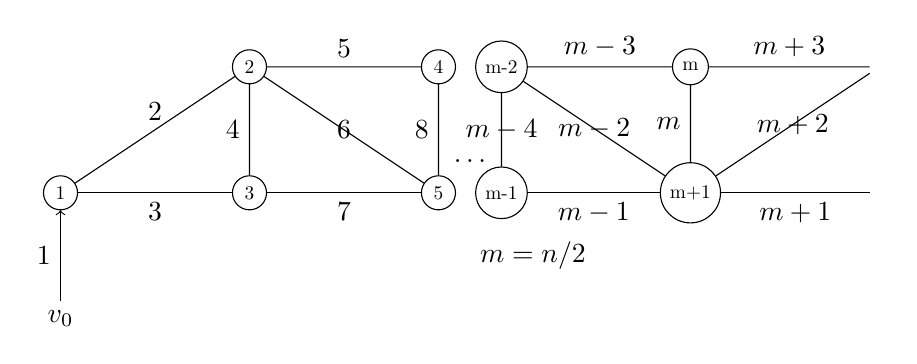
\begin{tikzpicture}[scale=0.8]

    \tikzset{nodestyle/.style={draw,shape=circle,scale=0.7}}
    \node[nodestyle] (p1) at ( 0, 0) {1}; 
    \node[nodestyle] (p2) at ( 3, 0) {3};
    \node[nodestyle] (p3) at ( 6, 0) {5};
    \node[nodestyle] (p33) at ( 7, 0) {m-1};
    \node[nodestyle] (p4) at ( 10, 0) {m+1};
    \node (p5) at ( 13, 0) {};

    \node[nodestyle] (p8) at ( 3, 2) {2};
    \node[nodestyle] (p9) at ( 6, 2) {4};
    \node[nodestyle] (p99) at ( 7, 2) {m-2};
    \node[nodestyle] (p10) at ( 10, 2) {m};
    \node (p11) at ( 13, 2) {};
    
    \node(pDots) at (6.5,0.5) {$\dots$};
    
    \begin{scope}[every path/.style={-}]
        \draw (p1) -- (p2) node[below,midway]{$3$};
        \draw (p2) -- (p3) node[below,midway]{$7$}; 
        \draw (p33) -- (p4) node[below,midway]{$m-1$};
        \draw (p4) -- (p5) node[below,midway]{$m+1$};


        \draw (p8) -- (p9) node[above,midway]{$5$};
        \draw (p99) -- (p10) node[above,midway]{$m-3$};
        \draw (p10) -- (p11) node[above,midway]{$m+3$};

        \draw (p1) -- (p8) node[above,midway]{$2$};

        \draw (p2) -- (p8) node[left,midway]{$4$};
        \draw (p3) -- (p9) node[left,midway]{$8$};
        \draw (p33) -- (p99) node[midway]{$m-4$};        
        \draw (p4) -- (p10) node[left,midway]{$m$};

        \draw (p8) -- (p3) node[midway]{$6$};
        \draw (p99) -- (p4)node[midway]{$m-2$};
        \draw (p4) -- (p11)node[midway]{$m+2$};
    \end{scope}  

    
    \node (v0) at ( 0, -2) {$v_0$};
    \node (aclaracion) at ( 7.5, -1) {$m = n/2$};

    %\begin{scope}[every path/.style={-}]
        \draw[->] (v0) -- (p1) node[left,midway]{$1$};
    %\end{scope}

        % Nodos artificiales.
         
\end{tikzpicture}